\documentclass[journal]{IEEEtran}
\usepackage{amsmath,amssymb}
\usepackage{booktabs}
\usepackage{graphicx}
\usepackage{url}
\usepackage{algorithm}
\usepackage{algpseudocode}
\usepackage{array}
\newcommand{\method}{VAST-GWO}

\begin{document}

\title{\method{}: A Verified Archive-Guided Sparse-Evaluation Grey Wolf
Optimizer for Global Optimization and 3D UAV Path Planning}

\author{Draft -- \texttt{sparse\_q} research branch\thanks{All experiments in
this manuscript come from the frozen batch recorded in the accompanying
repository; every reported number is reproducible from the archived runs, and
the evaluation counts of all runs are audited by an independent probe.}}

\maketitle

\begin{abstract}
Metaheuristic optimizers are increasingly deployed where each objective
evaluation is expensive, so the real-evaluation budget---not arithmetic---is
the resource that decides solution quality. The grey wolf optimizer (GWO)
spends this resource uniformly over the whole pack and drives search from three
leader wolves only, which invites premature convergence and makes each
evaluation less informative than it could be. This paper proposes
\method{}, a verified archive-guided sparse-evaluation GWO. In every
generation, 100 cheap candidates are generated from three complementary
routes: standard GWO leader moves (50), success-scale shells around the
current alpha wolf (12), and multi-region shells and two-centre segments
produced from a verified elite archive (38). Only $K=10$ uniformly sampled
candidates receive a real evaluation, and unevaluated candidates never
influence leaders, archives or rankings---a verified-state discipline that
keeps every piece of search memory backed by a billed evaluation. On CEC2017
at $D=50$ with 100{,}000 true evaluations and 30 independent runs,
\method{} ranks first among seven methods (mean rank 2.24), significantly
outperforming the 2026 hierarchical HAGWO, PSO, CLPSO, the 2026 adaptive
oppositional AOGWO and standard GWO, and reaching statistical parity with the
strong improved GWO. A controlled equal-slot ablation shows that the verified
archive carries the improvement---removing it degrades the method to 27 losses
in 29 functions, and replacing it with a single alpha-centred sampler
collapses it to 2 wins---while the alpha-shell route is optional once the
archive is present. In a 209-dimensional, DEM-based 3D UAV delivery
application with hard time windows, \method{} is the only method that finds
feasible routes in all 150 runs, attains the smallest censored mean time to
feasibility, and produces the best final route quality against every
baseline after Holm correction. These results indicate that, under limited
real-evaluation budgets, the structure of candidate sources matters more than
the complexity of the evaluation scheduler.
\end{abstract}

\begin{IEEEkeywords}
Grey wolf optimizer; sparse evaluation; verified elite archive; multi-region
search; limited evaluation budget; UAV path planning; CEC2017.
\end{IEEEkeywords}

\section{Introduction}
Nature-inspired optimizers are now a standard tool for engineering design,
scheduling and path planning, because they make few assumptions about the
objective and scale to black-box simulators. Their practical cost, however,
is dominated by the objective function itself: in finite-element calibration,
computational-fluid design or UAV mission planning a single evaluation may
take seconds to hours, so the total number of \emph{real} evaluations is the
binding constraint rather than the number of arithmetic operations
\cite{yu2021multimodel,liu2024survey,zhao2025surrogate}. Under such budgets,
an optimizer must answer one question well: \emph{where should the next real
evaluation be spent?}

The grey wolf optimizer (GWO) \cite{mirjalili2014gwo} is a particularly
attractive starting point: it is parameter-light, easy to implement and has
been applied across IoT, feature selection, agriculture and UAV planning
\cite{nadimishahraki2024iot,makhadmeh2023review}. Its classic form, however,
evaluates the entire pack every generation and derives all movement from the
three leaders ($\alpha$, $\beta$, $\delta$). When evaluations are scarce this
design has two consequences: budgets are consumed on candidates whose
information value is unknown, and the search distribution concentrates
around the same leaders, which is the classical route to premature
convergence and stagnation on multimodal landscapes.

A large recent literature improves GWO from different angles. Operator-level
variants add differential evolution and elimination
\cite{wang2019igwode}, mutation with evolutionary population dynamics
\cite{zhang2025mutation}, teaching--learning hybrids \cite{singh2025tlbo},
beetle-antennae hybrids \cite{zhang2025bagwo}, grey wolf--particle swarm
hybrids \cite{shaikh2025hybrid}, self-repulsion for feature selection
\cite{wang2025selfrepulsion} and improved engineering-oriented forms
\cite{li2021sustainability}. Learning-driven variants let reinforcement
learning or Q-learning choose update strategies or leaders
\cite{yin2026amsgwo,huang2026qlfdgwo,khalid2026aogwo,wang2026dmsgwo}, and
recent drones-specific versions target UAV trajectory planning
\cite{nayeem2025drones,jia2025drones}. These methods deliver strong results,
but they are typically tuned and compared under protocols in which every
individual is evaluated each generation or the budget is defined in
iterations. They also tend to stack mechanisms, so it is rarely isolated
\emph{which} design element produces the gain.

This paper takes the evaluation budget itself as the design constraint and
asks a deliberately narrow question: \emph{given a fixed number of real
evaluations per generation, how should the candidate pool be composed?} We
propose \method{} (Verified Archive-guided Sparse-evaluation Technique for
Grey Wolf Optimization), which separates cheap candidate generation from real
evaluation and admits information into the search state only after it has
been verified by a billed evaluation. The candidate pool combines three
routes---standard GWO moves, success-scale alpha shells, and multi-region
candidates drawn from a verified elite archive---and only a small random
subset of the pool is ever evaluated, which makes the composition of the pool
the decisive design variable.

The contributions of this paper are summarized as follows.

\begin{itemize}
\item \textbf{A verified-state sparse-evaluation framework.} Each generation
generates $M=100$ cheap candidates, evaluates $K=10$ of them under a strictly
audited true-evaluation budget, and lets no unevaluated candidate influence
leaders, archives, rankings or statistics.
\item \textbf{A verified multi-region archive as a candidate source.} The
archive stores only real-evaluated improvements, enforces a separation
threshold, and contributes shells around its centres and segments between
them. A controlled equal-slot ablation shows that this route is the main
performance engine: disabling the auxiliary routes reduces the method to
27 losses in 29 functions against the full version, and replacing the archive
with a single alpha-centred sampler collapses it to 2 wins in 29 functions.
\item \textbf{Complete evidence under one protocol.} A seven-method CEC2017
comparison at $D=50$ (29 functions, 30 seeds, 100{,}000 true evaluations),
a five-arm equal-slot source ablation, stagnation and early-budget probes,
and two additional resource tiers ($D=100$; 20{,}000 evaluations) are
reported with identical initial populations and probe-audited budgets.
\item \textbf{A demanding application.} On a 209-dimensional, DEM-based 3D
UAV delivery problem with hard time windows on five real terrain scenarios,
\method{} is the only method that finds feasible routes in all 150 runs, has
the smallest censored mean time to feasibility, and delivers the best final
route quality against every baseline after Holm correction.
\item \textbf{Design-space boundaries.} Directed screening, fixed exploration
quotas, three Q-learning quota schedulers, stagnation radius boosting and
success-direction steering are all tested with matched controls; none
improves on uniform random allocation, which shows that the gains come from
the candidate-source structure rather than from added scheduling complexity.
\end{itemize}

The remainder of this paper is organized as follows. Section~II reviews
related work. Section~III presents \method{}. Section~IV describes the
experimental protocol, Section~V reports the optimization results,
Section~VI the ablation and mechanism analysis, and Section~VII the UAV
application. Section~VIII discusses implications and scope, and Section~IX
concludes.

\section{Related Work}
\subsection{Grey wolf optimizer and its variants}
GWO \cite{mirjalili2014gwo} models the leadership hierarchy and cooperative
hunting of grey wolves: the three best solutions guide the pack through
encircling and attacking equations whose exploration--exploitation balance is
controlled by a linearly decreasing parameter. Comprehensive reviews document
its variants and applications in IoT and beyond
\cite{nadimishahraki2024iot,makhadmeh2023review}. Representative recent
improvements include differential-evolution and elimination mechanisms
\cite{wang2019igwode}, mutation with evolutionary population dynamics and
nonlinear population reduction \cite{zhang2025mutation}, teaching--learning
hybridization \cite{singh2025tlbo}, beetle-antennae search hybridization
\cite{zhang2025bagwo}, grey wolf--particle swarm hybrids
\cite{shaikh2025hybrid}, self-repulsion strategies \cite{wang2025selfrepulsion},
and engineering-oriented improved variants \cite{li2021sustainability}, as
well as improved GWO for general engineering design
\cite{nadimi2021igwo}. The strong improved GWO \cite{nadimi2021igwo} is used
as a baseline in this paper. Learning-driven variants couple GWO with
reinforcement learning or Q-learning for strategy, leader or quota selection
\cite{yin2026amsgwo,huang2026qlfdgwo,khalid2026aogwo,wang2026dmsgwo}, and
UAV-specific versions embed Q-learning or reinforcement learning into
trajectory planning \cite{nayeem2025drones,jia2025drones}. The present work
differs in that it neither adds a new update equation nor a learning
scheduler; it reorganizes \emph{which candidates exist} under a fixed number
of real evaluations per generation.

\subsection{Memory and archive mechanisms}
Memory is a recurring idea in swarm intelligence, where it stabilizes search
and preserves diversity. Recent GWO variants use elite memories, cross-search
memory or two-archive structures to handle large-scale or multi-objective
problems \cite{zamani2026egwo,tejani2025twoarchive}. \method{} shares the
motivation but differs in two respects. First, the archive is
\emph{verified}: only solutions that received a real evaluation may enter, so
the archive never stores a guess. Second, the archive is not only a
diversity reservoir---its centres and the segments between them directly
\emph{generate} candidates, which is the property that the ablation of
Section~VI isolates.

\subsection{Optimization under expensive evaluations}
When evaluations are expensive, surrogate-assisted evolutionary algorithms
are the dominant paradigm: models of the objective guide the search and are
updated with a limited number of real evaluations
\cite{yu2021multimodel,liu2024survey,zhao2025surrogate}. \method{} is
complementary rather than competing: it uses no surrogate, and it targets the
regime where each real evaluation is affordable but scarce enough that the
per-generation allocation must be fixed and audited. This makes the
comparison clean---every method receives exactly the same number of billed
evaluations---and it isolates candidate-source design from modelling effort.

\section{Proposed Method}
\subsection{Overview and verified-state discipline}
Fig.~\ref{fig:framework} shows one generation of \method{}. A candidate pool
of $M=100$ positions is generated from three routes without any objective
evaluation. Exactly $K=10$ pool members are then sampled uniformly at random
and evaluated with the real objective; each call is billed, and a runtime
probe asserts that the audited count equals the budget exactly. The evaluated
subset drives all state updates: the leaders $\alpha,\beta,\delta$, the
verified elite archive, and the statistics used by the routes. Unevaluated
candidates have no effect on any of them---the verified-state discipline.
The budget of 100{,}000 evaluations decomposes as 50 initialization
evaluations plus 9{,}995 generations of ten evaluations.

\begin{figure}[t]
\centering
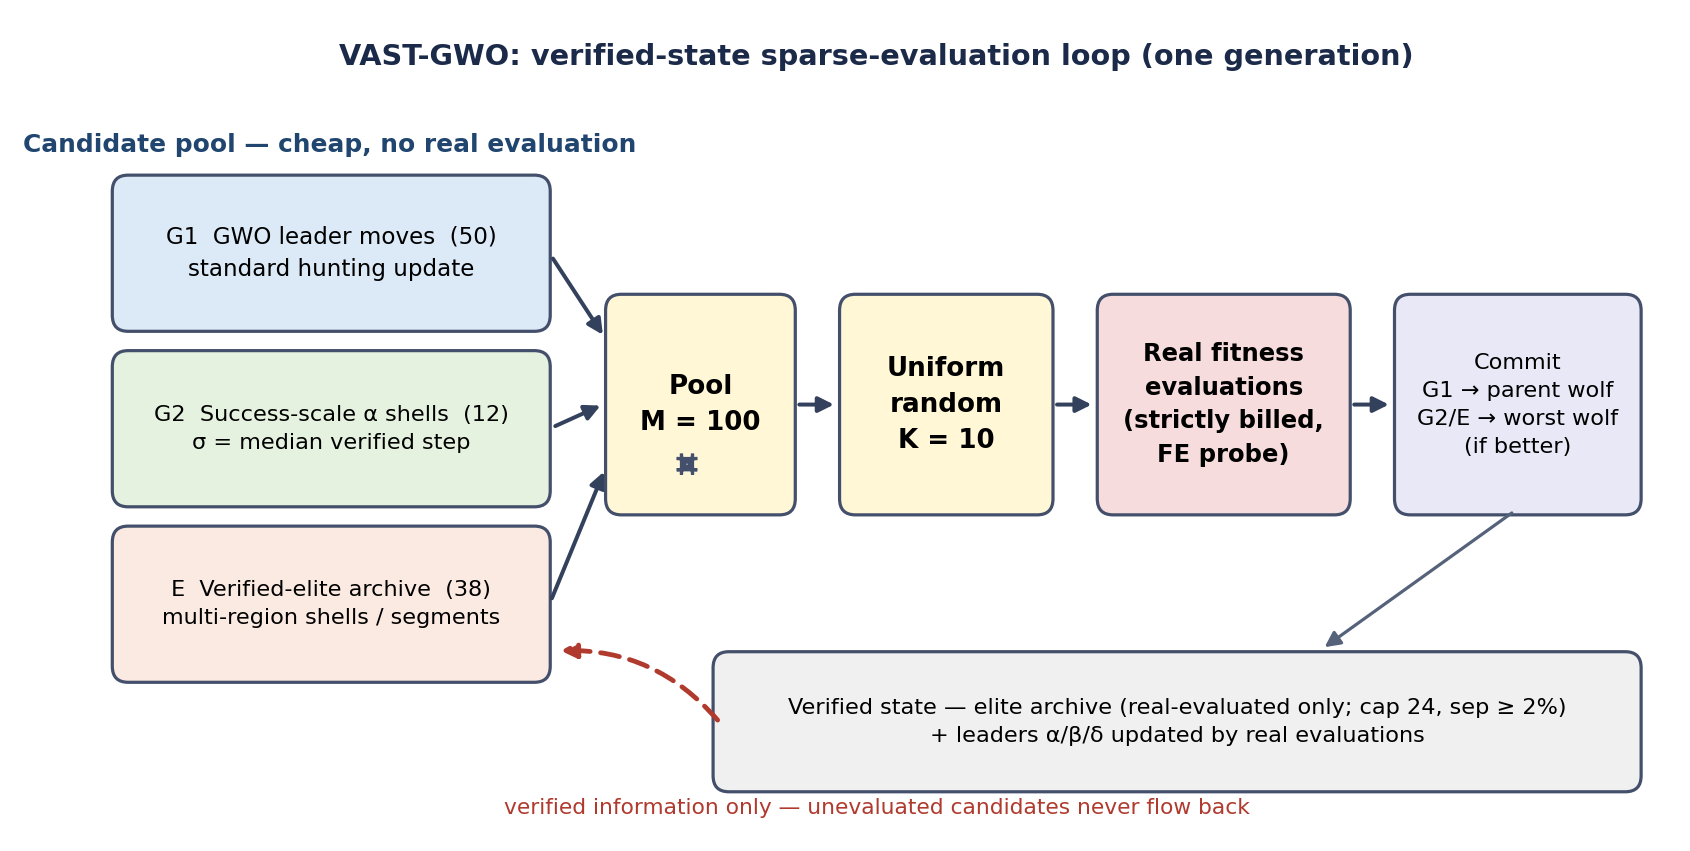
\includegraphics[width=\columnwidth]{figures/fig1_framework.png}
\caption{One generation of \method{}. A pool of 100 cheap candidates is
generated from three routes; only $K=10$ uniformly sampled candidates receive
a real (billed) evaluation, and only verified information flows back into the
leaders and the archive.}
\label{fig:framework}
\end{figure}

\subsection{Candidate generation routes}
\paragraph{G1: GWO leader moves (50 candidates).}
For each wolf $i$ the standard aggregation of the three leader-attracted
positions is formed,
\begin{equation}
X_i^{G1}=\tfrac{1}{3}\sum_{k\in\{\alpha,\beta,\delta\}}
\bigl(X_k - A_k \odot |C_k \odot X_k - X_i|\bigr),
\end{equation}
with $A_k=2a\,r_1-a$, $C_k=2r_2$, $r_1,r_2\sim U(0,1)^D$, and the
convergence factor $a=2-2\,\mathrm{FE}/\mathrm{FE}_{\max}$ driven by the true
evaluation count. This route preserves the classical hunting behaviour.

\paragraph{G2: success-scale alpha shells (12 candidates).}
Local refinement is generated in shells around the incumbent alpha wolf,
\begin{equation}
X^{G2}=X_\alpha+\sigma\odot(2u-1),\qquad
\sigma=\max\!\bigl(\mathrm{median}(\mathcal S_{25}),\;
0.01\,d_{\mathrm{diag}}\bigr),
\end{equation}
where $\mathcal S_{25}$ is the set of the 25 most recent \emph{verified}
successful step lengths (distances of accepted moves) and $d_{\mathrm{diag}}$
is the diagonal of the search space. The scale therefore adapts to the
observed geometry of successful moves instead of a fixed schedule.

\paragraph{E: verified elite archive (38 candidates).}
The archive stores up to 24 real-evaluated solutions whose objective values
improve the current worst archive member and whose distance to the nearest
stored solution exceeds $2\%$ of $d_{\mathrm{diag}}$; each entry carries a
credit that counts how often it has contributed to an accepted candidate.
Nineteen candidates are single-centre shells around credit-weighted archive
centres $c$,
\begin{equation}
X^{E_1}=c+\sigma\,(0.5+v)\odot(2u-1),
\end{equation}
and nineteen are two-centre segments between archive centres $c_1,c_2$,
\begin{equation}
X^{E_2}=c_1+\lambda\,(c_2-c_1)
+0.25\,\sigma\odot(2u-1),\quad
\lambda\sim U(0.15,0.85).
\end{equation}
Because archived centres are separated by construction, this route proposes
candidates in several distinct regions of the search space simultaneously---the
mechanism that the ablation in Section~VI identifies as the source of the
method's advantage.

\subsection{Sparse allocation and commit rules}
The $K=10$ evaluated candidates are drawn uniformly at random from the pool
without replacement, which keeps the allocation free of additional
hyperparameters and, as Section~VI shows, is not improved upon by screening,
quota or learning-based alternatives. Commits follow the origin of the
candidate: an evaluated G1 candidate replaces its parent wolf if it improves
that parent's objective; an evaluated G2 or E candidate replaces the current
worst wolf if it is strictly better. All accepted moves are appended to the
verified-step record that drives $\sigma$, and the archive and leaders are
updated exclusively from these evaluated results.

\subsection{Algorithm and complexity}
Algorithm~\ref{alg:vast} summarizes the procedure. Per generation the method
performs $M=100$ cheap candidate constructions of cost $O(MD)$ and $K=10$
objective evaluations; the archive and shell statistics add $O(|\mathcal
A|D)$ with $|\mathcal A|\le 24$. Relative to standard GWO, which evaluates
$N=50$ candidates per generation, the arithmetic overhead of the pool is
modest while the number of billed evaluations per generation drops by a
factor of five; the wall-clock comparison at equal budgets is reported in
Section~V-D.

\begin{algorithm}[t]
\caption{\method{} (one run)}
\label{alg:vast}
\begin{algorithmic}[1]
\State initialize $N$ wolves by real evaluation; set
$\alpha,\beta,\delta$ and $\mathcal A\!\leftarrow\!\emptyset$;
$\mathrm{FE}\!\leftarrow\!N$
\While{$\mathrm{FE}<\mathrm{FE}_{\max}$}
  \State build pool: 50 G1 moves (Eq.~1), 12 G2 shells (Eq.~2), 38 archive
  candidates (Eqs.~3--4)
  \State sample $K=10$ candidates uniformly without replacement
  \For{each sampled candidate $x$}
     \State $f(x)\leftarrow$ real evaluation; $\mathrm{FE}\!\mathrel{+}\!=\!1$
     \State commit $x$ according to its route (parent or worst wolf, if better)
     \State update verified-step record, archive and
     $\alpha,\beta,\delta$ from verified results only
  \EndFor
\EndWhile
\State \Return best verified solution
\end{algorithmic}
\end{algorithm}

\section{Experimental Setup}
\paragraph{Benchmark and protocol.}
All optimization experiments use the CEC2017 benchmark suite with
F1 and F3--F30 (29 functions; the official package omits F2), dimension
$D=50$, $100{,}000$ true evaluations, and 30 independent runs (seeds
3001--3030). Every algorithm receives the same initial population for each
(function, seed) pair; the initialization random stream and the search random
stream are separated. All batches run on MATLAB with exactly four parallel
workers, atomic per-run storage and resumable execution, and an independent
probe asserts that each run consumes exactly its budget
\cite{awad2016problem}. An out-of-sample seed block (3071--3100) is used only
for the ablation study.

\paragraph{Baselines.}
The comparison set contains six methods, all implemented or audited in the
same codebase: standard GWO \cite{mirjalili2014gwo}; the strong improved GWO
\cite{nadimi2021igwo}; HAGWO \cite{su2026hagwo}; classic PSO with linearly
decreasing inertia \cite{kennedy1995pso,shi1998modified}; CLPSO
\cite{liang2006clpso}; and AOGWO \cite{khalid2026aogwo}. Baseline-specific
parameters are summarized in Table~\ref{tab:params}.

\begin{table}[t]
\centering
\small
\caption{Baseline configurations (identical budget for all methods).}
\label{tab:params}
\begin{tabular}{ll}
\toprule
Method & Configuration \\
\midrule
GWO & $N=50$ \\
I-GWO & $N=50$, as published \\
HAGWO & $N=50$, as published \\
PSO & $N=50$, $w$: 0.9$\to$0.4, $c_1=c_2=2$, $v_{\max}=0.2\,r$ \\
CLPSO & $N=50$, $P_c$ schedule and refresh as published \\
AOGWO & $N=50$, as published \\
\bottomrule
\end{tabular}
\end{table}

\paragraph{Statistics.}
For every baseline, per-function paired Wilcoxon tests on identical seeds are
reported together with Holm correction, the median paired error ratio
(baseline over \method{}), function-mean win--loss counts and the mean rank
over the 29 functions. Pooled paired tests are reported for completeness but
are not used as primary evidence. The same protocol applies to the ablation
and to the application study.

\section{Results}
\subsection{Comparison with strong baselines}
Table~\ref{tab:main} reports the final seven-method comparison. \method{}
attains mean rank 2.24---first among the seven methods---ahead of the strong
improved GWO (2.28), the 2026 hierarchical HAGWO (3.41), PSO (4.41), CLPSO
(4.48), the 2026 adaptive oppositional AOGWO (5.07) and standard GWO (6.10).
Against standard GWO the improvement is decisive: 28 wins in 29 functions,
median ratio 0.525, Holm $+24/-0$. Against HAGWO, PSO, CLPSO and AOGWO the
margins are statistically significant (see Table~\ref{tab:main}), and against
the strong improved GWO the comparison is a statistical tie (ratio 0.938,
17--12, pooled $p=0.55$) with large function-level swings in both directions
(e.g.\ $7\times$ better on F1 and $140\times$ on F9). The claim this
comparison supports is therefore precise: \method{} is the best-ranked
method in the set and is significantly better than five of six baselines,
while remaining statistically indistinguishable from the strongest classical
improvement.

\begin{table}[t]
\centering
\small
\caption{Final seven-method comparison (CEC2017, $D=50$, 100{,}000 true
evaluations, 29 functions, 30 runs, identical seeds). ``Med.\ ratio'' is the
median paired error ratio of \method{} over each baseline (below one favours
\method{}); Holm counts per-function significant wins/losses after Holm
correction.}
\label{tab:main}
\resizebox{\columnwidth}{!}{\begin{tabular}{lrrrrr}
\toprule
Method & Med.\ ratio & W-L & Holm $+/-$ & Pooled $p$ & Mean rank\\
\midrule
\textbf{VAST-GWO} & -- & -- & -- & -- & \textbf{2.24}\\
I-GWO & 0.938 & 17-12 & $+12/-6$ & 0.55 & 2.28\\
HAGWO (2026) & 0.806 & 22-7 & $+19/-3$ & $2.2\times10^{-36}$ & 3.41\\
PSO & 0.652 & 23-6 & $+19/-2$ & $5.8\times10^{-31}$ & 4.41\\
CLPSO & 0.668 & 21-8 & $+20/-5$ & $7.4\times10^{-27}$ & 4.48\\
AOGWO (2026) & 0.586 & 27-2 & $+21/-0$ & $1.3\times10^{-85}$ & 5.07\\
GWO & 0.525 & 28-1 & $+24/-0$ & $6.7\times10^{-103}$ & 6.10\\
\bottomrule
\end{tabular}
}
\end{table}

\begin{figure}[t]
\centering
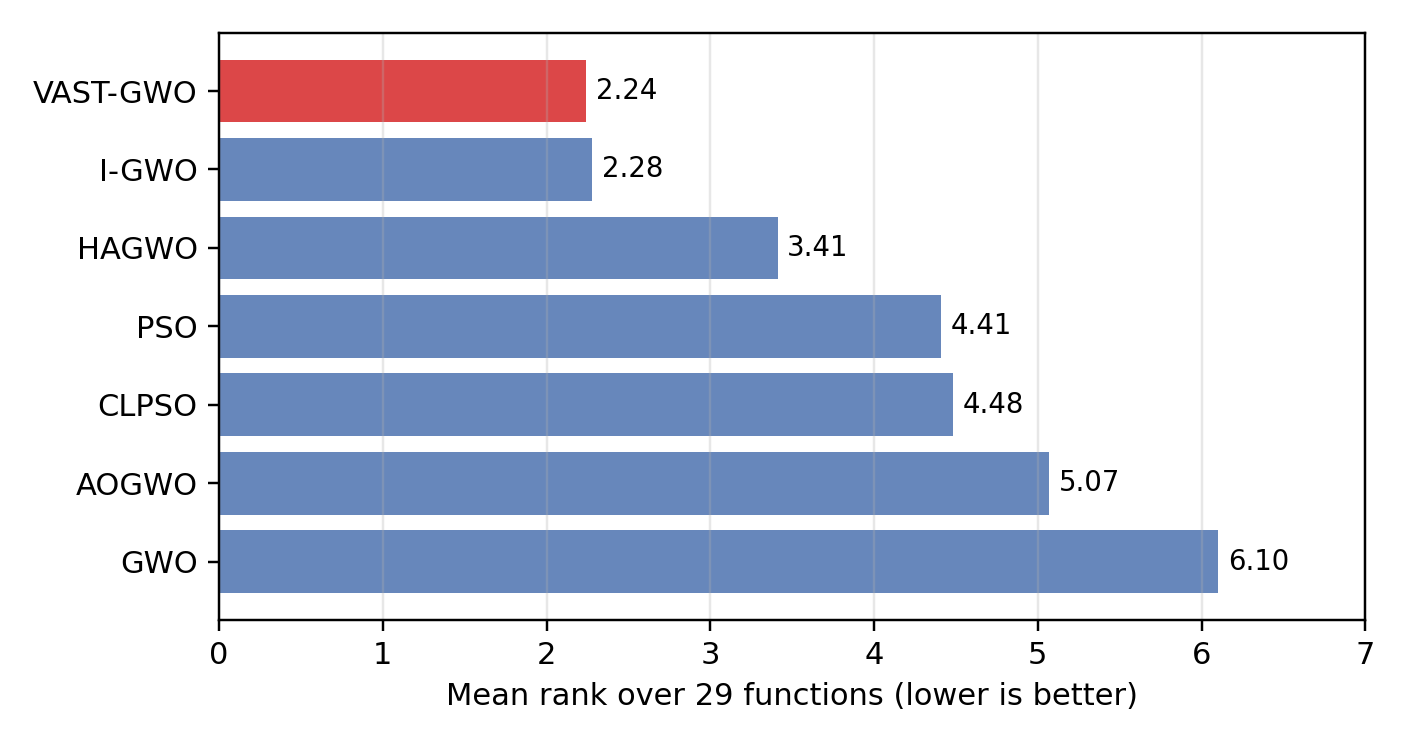
\includegraphics[width=\columnwidth]{figures/ranks7.png}
\caption{Mean ranks over the 29 CEC2017 functions for the final seven-method
comparison ($D=50$, 100{,}000 true evaluations, 30 runs each).}
\label{fig:ranks}
\end{figure}

\subsection{Early-budget behaviour and exploration}
The advantage appears early and grows with the budget. At 10\%, 20\% and 50\%
of the evaluation budget the median error ratios against standard GWO are
0.802, 0.777 and 0.726, with 25, 26 and 27 wins out of 29 functions,
respectively. Against the frozen full-evaluation ANGWO reference the ratios
are 0.732 and 0.768 at 10\% and 20\%, and the simple-multimodal subset
(F4--F10) reaches a ratio of 0.714. The probe-instrumented behaviour table
(Table~\ref{tab:behaviour}) shows the same picture from the search dynamics:
\method{} recovers from stagnation windows more often than GWO
(0.823 vs.\ 0.757) and spends less of the budget in long stagnation
(0.813 vs.\ 0.844); its useful-novelty rate---evaluations that are both novel
and convert into improvements---is 0.0064 versus 0.0035 for GWO. The
improving-evaluation rate itself is lower (0.0031 vs.\ 0.0048), consistent
with a search that places fewer, better-targeted evaluations.

\begin{table}[t]
\centering
\small
\caption{Behaviour metrics on the formal tier (probe-instrumented methods).}
\label{tab:behaviour}
\resizebox{\columnwidth}{!}{\begin{tabular}{lrrrrr}
\toprule
Method & Recovery prob. & Long-stag.\ share & Useful novelty & Nov.\ rate Q4 & Impr.\ rate Q4\\
\midrule
S-star & 0.823 & 0.813 & 0.00640 & 0.712 & 0.00308 \\
S1-pool38 & 0.816 & 0.812 & 0.00590 & 0.695 & 0.00266 \\
S3p-q25 & 0.808 & 0.821 & 0.00563 & 0.745 & 0.00272 \\
S5p-q & 0.780 & 0.835 & 0.00629 & 0.716 & 0.00264 \\
B0-ANGWO & 0.768 & 0.831 & 0.00578 & 0.690 & 0.00447 \\
GWO & 0.757 & 0.844 & 0.00347 & 0.588 & 0.00481 \\
\bottomrule
\end{tabular}}
\end{table}

\subsection{Scalability and resource-constrained tiers}
Two additional tiers confirm that the advantage is not tied to one operating
point. At $D=100$ (29 functions, ten seeds, 100{,}000 evaluations)
\method{} again ranks first (mean rank 1.72 versus 2.00, 2.33, 3.52 and 3.67
for the compared variants), with a 0.703 median ratio and 10 wins against 2
losses (Holm $+5/-1$) on the 12-function subset shared with the improved GWO.
Under a five-times-smaller budget (20{,}000 evaluations, 29 functions, ten
seeds) it ranks first as well (1.97 versus 2.31 and 3.83 for the compared
variants), winning 24 of 29 functions against standard GWO (ratio 0.721) and
24 of 29 against the frozen ANGWO reference (0.807). The sparse framework
therefore scales upward in dimension and downward in budget.

\subsection{Runtime}
At equal budgets \method{} is the most expensive method in wall-clock terms
(5.93~s per run at $D=50$/100{,}000 evaluations, versus 3.63~s for GWO,
3.41~s for HAGWO, 2.59~s for PSO, 2.41~s for CLPSO, 2.32~s for I-GWO and
4.54~s for AOGWO). This is the transparent price of building and maintaining
a 100-candidate pool and a verified archive with a limited number of actual
evaluations, and it is reported here so that practitioners can weigh quality
against time.

\section{Ablation and Mechanism Analysis}
\subsection{Where the performance comes from}
The ablation replaces disabled routes by additional standard GWO candidates
so that the pool size ($M=100$), the evaluated subset ($K=10$) and the
budget remain identical; the full configuration is bitwise identical to the
frozen implementation on audited samples. Table~\ref{tab:ablation} reports
the outcome. Removing both auxiliary routes (A0: GWO-only sparse pool)
degrades the method to 27 losses in 29 functions (ratio 0.538, Holm
$+23/-0$), which shows that sparse evaluation alone is not the source of the
advantage. Removing the archive while keeping the alpha shells (A1) degrades
the method to 25 losses (0.812, Holm $+21/-1$). Keeping the archive but
removing the alpha shells (A2) leaves performance statistically unchanged
(0.994, 14--15, pooled $p=0.326$), i.e.\ the alpha-shell route is optional
once the archive is present. Finally, replacing the archive by a single
alpha-centred sampler with identical slots, scale and acceptance rule (A5)
collapses the method to 2 wins in 29 functions (ratio 1.407, Holm
$+2/-23$). The mechanism conclusion is therefore sharp: \emph{the verified
multi-region archive is the performance engine of \method{}}, and the route
structure, not the amount of sparse evaluation, is what must be engineered.

\begin{table}[t]
\centering
\small
\caption{Equal-slot candidate-source ablation (29 functions, 30 seeds,
100{,}000 true evaluations, seeds 3071--3100). Ratios are relative to the
full configuration; Holm counts significant wins/losses of the listed
comparison.}
\label{tab:ablation}
\begin{tabular}{lrrrr}
\toprule
Comparison & Med.\ ratio & W-L & Holm $+/-$ & Pooled $p$\\
\midrule
Full vs A0 (GWO-only pool) & 0.538 & 27-2 & $+23/-0$ & $7\times10^{-102}$\\
Full vs A1 (G1+G2) & 0.812 & 25-4 & $+21/-1$ & $5\times10^{-60}$\\
Full vs A2 (G1+E) & 0.994 & 14-15 & $+1/-0$ & 0.326\\
A2 vs A0 & 0.510 & 29-0 & $+27/-0$ & $7\times10^{-117}$\\
A5 (alpha-centred) vs Full & 1.407 & 2-27 & $+2/-23$ & $1\times10^{-64}$\\
\bottomrule
\end{tabular}
\end{table}

\subsection{Source-level attribution}
Instrumenting every commit with its route explains the ablation at the level
of accepted moves: in a full run the archive route accounts for about 24{,}100
accepted real improvements per run on average, compared with about 11{,}300
for the GWO-move route and 4{,}700 for the alpha-shell route
(Fig.~\ref{fig:sources}). The archive route is thus not only present more
often in the winning configuration; it is the route that actually converts
evaluations into progress.

\begin{figure}[t]
\centering
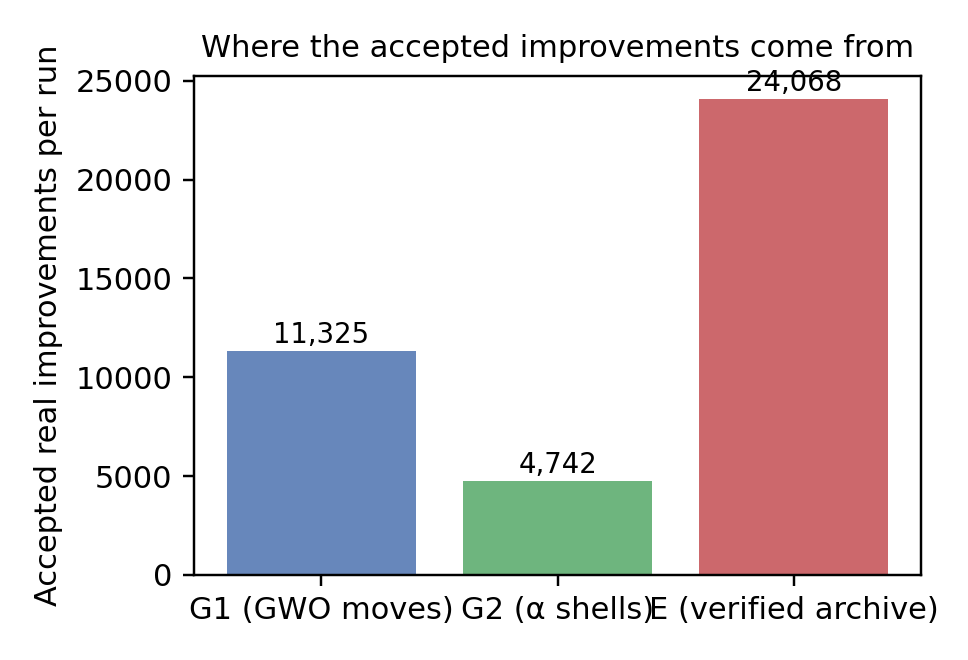
\includegraphics[width=0.85\columnwidth]{figures/fig4_sources.png}
\caption{Accepted real improvements per run by candidate route (mean over the
formal ablation batch). The verified archive route dominates; the alpha-shell
route is the smallest contributor, consistent with its optional role once the
archive is present.}
\label{fig:sources}
\end{figure}

\subsection{Design-space boundaries}
The same controlled protocol was used to test the natural alternatives to
uniform random allocation and to two popular enhancement strategies. Directed
screening by incumbent geometry and history-informed selection were both
worse than uniform sampling in development tests (ratios 1.39 and 1.53);
fixed exploration quotas above the pool share degraded performance (up to
1.67); and three Q-learning quota schedulers never exceeded the best fixed
policy (ratios 0.99--1.13) although they consistently beat random quota
perturbation (0.75--0.87). A stagnation-triggered radius boost degraded
performance (1.20). Finally, success-direction steering---extending moves
along previously successful directions---improved final error against the
frozen configuration (22--7, Holm $+2/-0$) but an equal-magnitude
random-direction control achieved the same effect (ratio 0.988, pooled
$p=0.155$), and the gain appeared only in the last 20\% of the budget, so the
mechanism was rejected as an information-driven contribution. Together these
boundaries support a simple design rule under scarce real evaluations:
strengthen the \emph{sources} of candidates and keep the allocation simple.

\section{Application: 3D UAV Delivery Path Planning}
\subsection{Scenario and protocol}
The application is a three-dimensional UAV delivery problem built on five
real Copernicus DEM terrain tiles (ridge, peaks, mountain, hills, plateau).
Each instance contains 20 delivery stations with hard time windows, three
cylindrical threat zones, and three intermediate control points per flight
leg, giving a 209-dimensional mixed route-and-trajectory search space; the
objective combines flight distance, waiting time and path smoothness under
terrain-clearance, obstacle, altitude, climb-angle and turn-angle
constraints. This is a normalized simulation derived from real terrain data,
not a flight test. All methods run with $N=50$, 30{,}000 true evaluations
(initialization included), identical initial populations per (map, seed), and
30 seeds; 900/900 runs completed with zero failures.

\subsection{Reliability under a censoring horizon}
Table~\ref{tab:uav} reports reliability and quality. \method{} is the only
method that finds a feasible route in every one of its 150 runs; the runner-up
reliability is 97.3\% (I-GWO and HAGWO), followed by PSO (95.3\%), GWO
(94.0\%) and CLPSO (61.3\%). Because unsuccessful runs would otherwise make
median time-to-feasibility optimistic, we report the restricted mean time to
first feasibility (RMST) with a 30{,}000-evaluation censoring horizon, in
which every run---successful or not---enters the statistic. \method{} attains
the smallest RMST (7{,}062 evaluations, 95\% CI 6{,}449--7{,}731), ahead of
HAGWO (8{,}133) and PSO (8{,}138); the cumulative feasibility curves
(Fig.~\ref{fig:uavfeas}) show the same ordering developing from the middle of
the budget onwards, with 82.0\% feasibility at 10{,}000 evaluations and
100\% at 20{,}000 for \method{}.

\begin{table}[t]
\centering
\small
\caption{3D UAV delivery application (150 runs per method). Feas.: routes
found within 30{,}000 evaluations; RMST: censored mean time to first
feasibility (lower is better); costs are medians over feasible runs.}
\label{tab:uav}
\begin{tabular}{lcccc}
\toprule
Method & Feas.\ (\%) & RMST & First feas. & Cost \\
\midrule
\method{} & \textbf{100.0} & \textbf{7062} & 6314 & 667.4 \\
GWO & 94.0 & 10936 & 8920 & 699.8 \\
I-GWO & 97.3 & 12270 & 11152 & 724.7 \\
HAGWO & 97.3 & 8133 & 7432 & 663.4 \\
PSO & 95.3 & 8138 & 5357 & 766.4 \\
CLPSO & 61.3 & 24427 & 21330 & 1015.4 \\
\bottomrule
\end{tabular}
\end{table}

\begin{figure}[t]
\centering
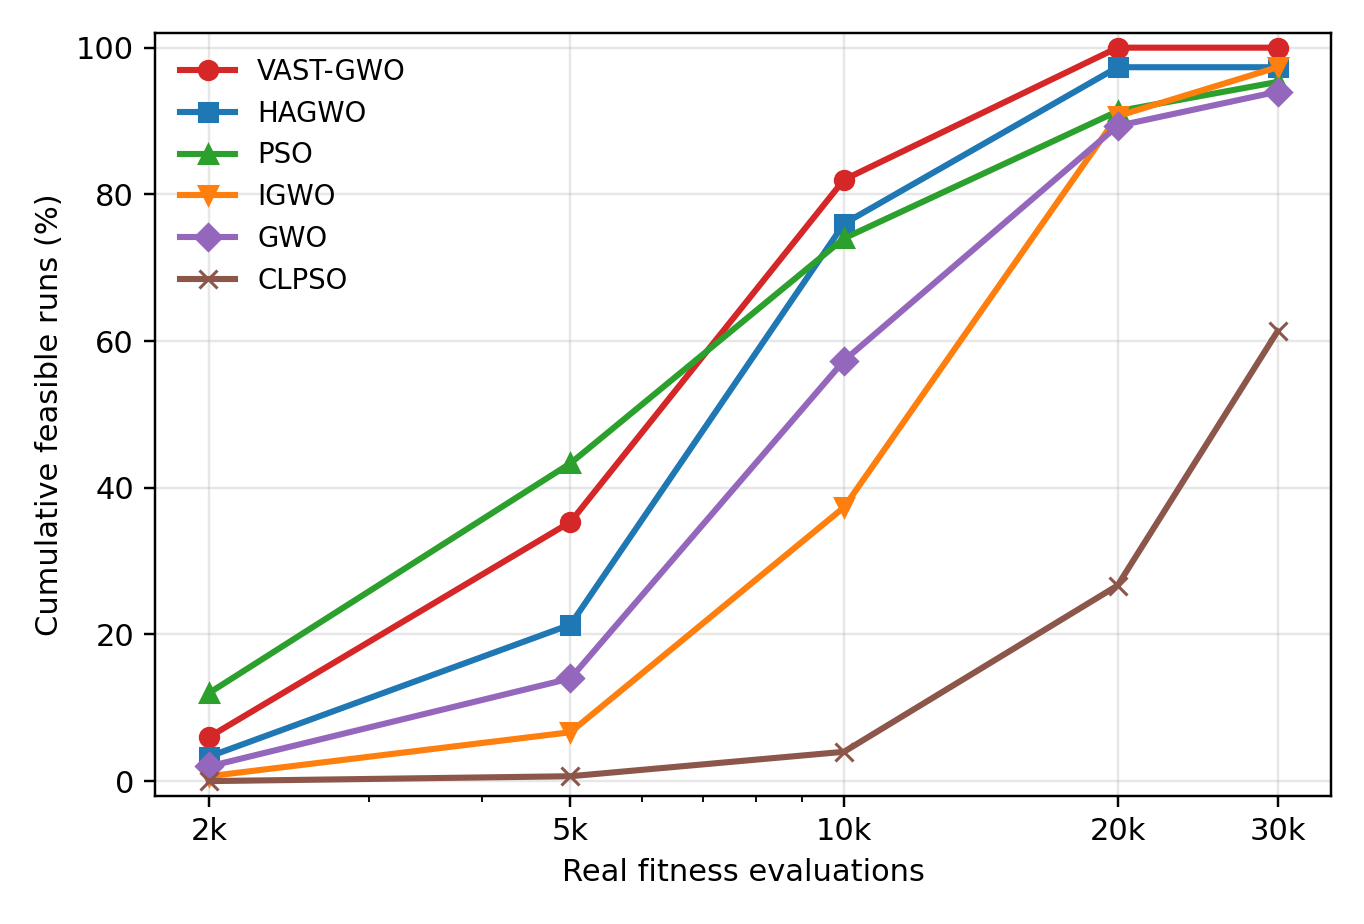
\includegraphics[width=\columnwidth]{figures/uav_feasibility_curve.png}
\caption{Cumulative feasible runs versus real evaluations on the five
DEM-based delivery scenarios (150 runs per method). Checkpoints are early
observations within the single 30k protocol.}
\label{fig:uavfeas}
\end{figure}

\begin{figure}[t]
\centering
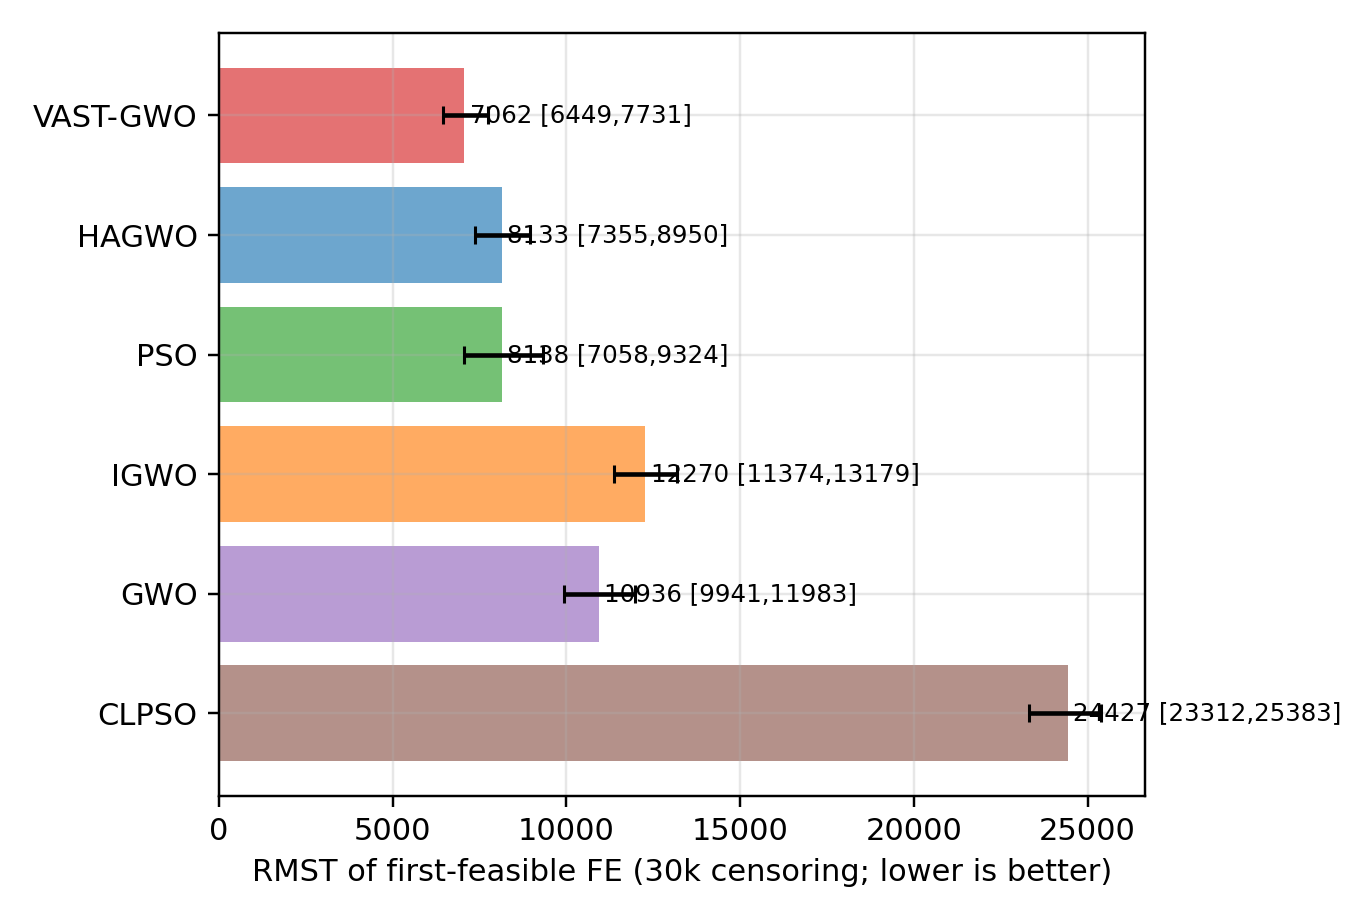
\includegraphics[width=\columnwidth]{figures/uav_rmst_bar.png}
\caption{Censored mean time to first feasible route (RMST, 30k horizon,
bootstrap 95\% CI). Every run enters the statistic.}
\label{fig:uavrmst}
\end{figure}

\subsection{Route quality and paired tests}
Final route quality favours \method{} against every baseline after Holm
correction over the five baselines: median paired ratios range from 0.631
(CLPSO) to 0.967 (HAGWO), with Holm $p$ from $3.3\times10^{-16}$ to
$0.0458$. The McNemar tests on final feasibility are significant against
GWO, PSO and CLPSO; against I-GWO and HAGWO the observed reliability
advantage is not significant with four discordant pairs, which we report for
completeness. Two comparisons deserve explicit reading. First, PSO finds
feasible routes earlier in the first few thousand evaluations (median 5{,}357
vs.\ 6{,}314), and its paired time-to-feasibility difference is not
significant ($p=0.598$ on the checkpoint-ordered test); in exchange, its
final routes are markedly worse (median cost 766.4 vs.\ 667.4) and it misses
feasibility in 7 of 150 runs. Second, HAGWO's marginal median cost (663.4) is
slightly below that of \method{} (667.4) because it conditions on its own
successful runs; on the 146 pairs where both methods succeed, \method{} is
significantly better (ratio 0.967, rank-biserial 0.19, Holm $p=0.0458$), and
it is fully reliable. Fig.~\ref{fig:uavroutes} shows the best route found by
\method{} on each of the five scenarios.

\begin{figure*}[t]
\centering
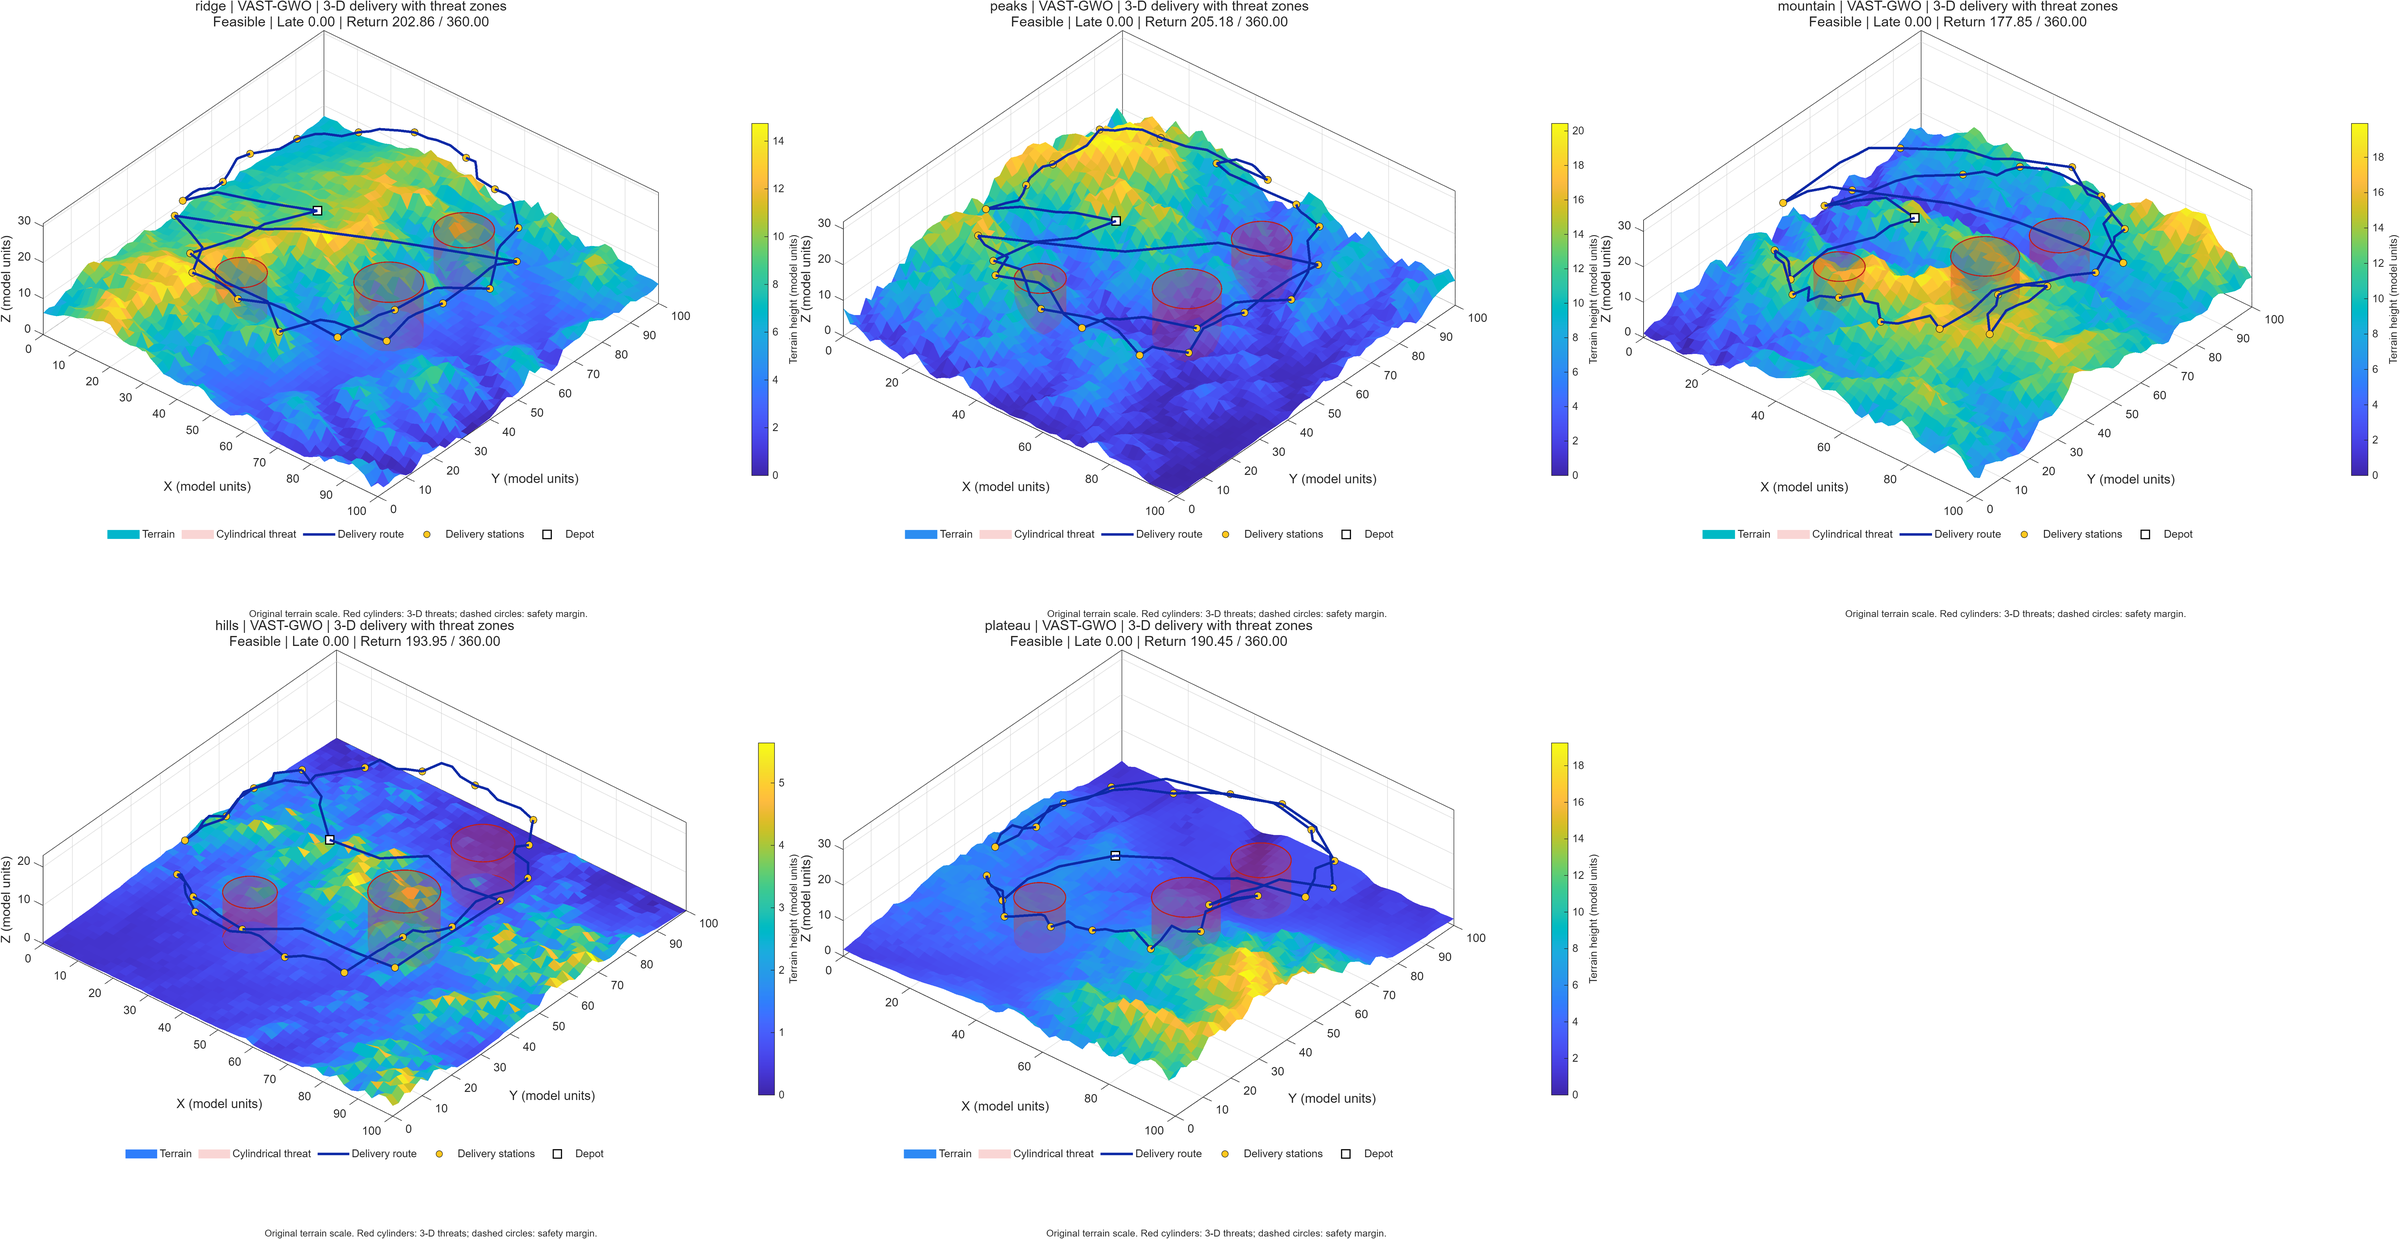
\includegraphics[width=\textwidth]{figures/uav_routes_montage.png}
\caption{Best feasible delivery routes found by \method{} on the five
DEM-based scenarios (costs 481.7--600.7). Terrain colour encodes elevation;
red cylinders are threat zones with safety margins; the blue polyline is the
route, dots are stations and the square is the depot.}
\label{fig:uavroutes}
\end{figure*}

\section{Discussion}
The experiments support a compact statement about optimizer design under
scarce real evaluations: \emph{the composition of the candidate pool is a
first-class design variable, and it can outperform additional scheduling
complexity}. In \method{} this composition is a verified archive spanning
several regions of the search space. Because every archived centre is backed
by a billed evaluation, the archive can safely generate candidates far from
the current leaders without introducing unverified optimism; because it
spans multiple regions, it counteracts the leader-driven contraction that
makes GWO stagnate on multimodal landscapes; and because the allocation
remains a simple uniform draw, none of the gains depend on a fragile
scheduler, as the boundary experiments confirm. The ablation makes the same
point from the opposite direction: once the archive is present, the
alpha-shell route is optional, and a single-centre substitute for the
archive destroys performance---multi-region verified memory, not local
refinement, is what the sparse budget needs.

Two properties recommend \method{} for practice. First, its behaviour is
robust across operating points: it ranks first both at $D=100$ and under a
budget five times smaller. Second, it transfers to a demanding constrained
application without re-tuning: on the 209-dimensional UAV delivery problem
it is the only method that is feasible in every run, and it combines this
reliability with the best censored time-to-feasibility and the best final
route quality against all baselines.

Scope and future work. The present study covers the CEC2017 family at
$D=50$/$D=100$ plus one application family (terrain-constrained 3D
delivery); extending the evidence to further engineering domains and to
higher dimensions is a natural next step, and surrogate coupling---using the
verified archive as training data for a lightweight model---is a promising
direction that the verified-state discipline makes particularly clean. The
ablation additionally indicates that a simplified variant that keeps only
the GWO-move and archive routes is a worthwhile subject for future study,
since the alpha-shell route was found optional in the presence of the
archive.

\section{Conclusion}
This paper introduced \method{}, a verified archive-guided sparse-evaluation
grey wolf optimizer for optimization under limited real-evaluation budgets.
The method separates cheap candidate generation (100 candidates from GWO
moves, success-scale alpha shells and a verified multi-region elite archive)
from real evaluation (ten uniformly sampled candidates per generation), and
admits only verified information into leaders, archives and rankings. On
CEC2017 at $D=50$ with 100{,}000 true evaluations and 30 seeds, \method{}
ranks first among seven methods, significantly outperforming five of six
baselines including the 2026 hierarchical HAGWO and the 2026 adaptive
oppositional AOGWO, while reaching statistical parity with the strongest
classical improvement. Controlled equal-slot ablations show that the verified
archive is the performance engine, and additional operating points
($D=100$; 20{,}000 evaluations) confirm the ranking. In a 209-dimensional
DEM-based 3D UAV delivery application with hard time windows, \method{} is
the only method feasible in all 150 runs and achieves both the best censored
time-to-feasibility and the best final route quality against every baseline.
The broader lesson is that under scarce real evaluations, engineering the
sources of candidates---and verifying everything that enters memory---pays
off more than engineering the scheduler.

\section*{Data and Code Availability}
All optimization and application experiments, including raw per-run records,
the experiment registry (every configuration and negative result), the
ablation implementation, the UAV scenarios and the analysis scripts, are
available in the accompanying repository; the evaluation counts of all runs
are asserted by an independent probe, and the frozen method configuration is
bitwise audited against its archived implementation.

\bibliographystyle{IEEEtran}
\bibliography{references}

\end{document}
